\section{Introduction}\label{intro}

In 1942, when anti-intellectualism was rising and the integrity of science was under attack, Robert K.\ Merton formulated four `institutional imperatives' as comprising the ethos of modern science: \emph{universalism}, meaning that the acceptance or rejection of claims entering the lists of science should not depend on personal or social attributes of the person bringing in these claims; \emph{``communism''} [sic], meaning that there should be common ownership of scientific findings and one should communicate findings, rather than keeping them secret; \emph{disinterestedness}, meaning that scientific integrity is upheld by not having self-interested motivations, and \emph{organized skepticism}, meaning that judgment on the scientific contribution should be suspended until detached scrutiny is performed, according to institutionally accepted criteria~\citep{merton1942science}. While the Mertonian norms may not formally be known to academics today, they still are implicitly being subscribed to in many ways in which academia has organized academic scrutiny; e.g., through the adoption of double-blind peer reviewing, and in motivations behind open science reforms.

At the same time, in the way in which academic research is disseminated in the AI and machine learning fields today, major shifts are happening. Where these research fields have actively adopted early sharing of preprints and code, the volume of publishable work has exploded to a degree that one cannot reasonably keep up with broad state-of-the-art, and social media influencers start playing a role in article discovery and citeability~\citep{weissburg2024tweets}. Furthermore, because of major commercial stakes with regard to AI and machine learning technology, and e.g.\ following the enthusiastic societal uptake of products employing large language models (LLMs), such as ChatGPT, the pressure to beat competitors as fast as possible is only increasing, and strong eagerness can be observed in many domains to `do something with AI' in order to innovate and remain current.

Where AI used to be a computational modeling tool to better understand human cognition~\citep{vanrooij2023aitheoretical}, the recent interest in AI and LLMs has been turning into one in which AI is seen as a tool that can mimic, surpass and potentially replace human intelligence. In this, the achievement of Artificial General Intelligence (AGI) has become a grand challenge, and in some cases, an explicit business goal. The definition of AGI itself is not as clear-cut or consistent; loosely, it is a phenomenon contrasting with `narrow AI' systems, that were trained for specific tasks~\citep{goertzel2014artificial}. In practice, to demonstrate that the achievement of AGI may be getting closer, researchers have sought to show that AI models generalize to different (and possibly unseen) tasks, with little human intervention, or show performance considered `surprising' to humans.

For example, Google DeepMind claimed their AlphaGeometry model~\citep{trinh2024geometry} reached a `milestone' towards AGI. This model has the ability to solve complex geometry problems, allegedly without the need for human demonstrations during training. However, work such as this had been initially introduced in the 1950s~\citep{hector2024linkedin}: without the use of an LLM, logical inference systems proved 100\% accurate in proving all the theorems of Euclidean Geometry, due to geometry being an axiomatically closed system. Therefore, while DeepMind created a powerfully fast geometry-solving machine, it is still far from AGI.

Generally, in the popularity of ChatGPT and the integration of generative AI in productivity tools (e.g.\ through Microsoft's Copilot integrations in GitHub and Office applications), one also can wonder whether the promise of AI is more in computationally achieving general intelligence, or rather in the engineering of general-purpose tools\footnote{A Swiss army knife is an effective general-purpose tool, without people wondering whether it is intelligent.}. Regardless, stakes and interests are high, e.g.\ with ChatGPT clearing nearly \$1 billion in months of its release\footnote{\url{https://www.bloomberg.com/news/articles/2023-08-30/openai-nears-1-billion-of-annual-sales-as-chatgpt-takes-off}}.

When combining massive financial incentives with the presence of a challenging and difficult-to-understand technology, that aims towards human-like problem-solving and communication abilities, a situation arises that is fertile for the misinterpretation of spurious cues as hints towards AGI, or other qualities like sentience\footnote{\url{https://www.scientificamerican.com/article/google-engineer-claims-ai-chatbot-is-sentient-why-that-matters/}} and consciousness. AI technology only becomes more difficult to understand as academic publishing in the space largely favors performance, generalization, quantitative evidence, efficiency, building on past work, and novelty~\citep{values_in_ML}. As such, works that make it into top-tier venues tend to propose heavier and more complicated technical takes on tasks that (in the push towards generalizability) get more vague, while the scaling-up of data makes traceability of possible memorization harder. In a submission-overloaded reality, researchers may further get incentivized to oversell and overstate achievement claims.

Noticing these trends, we as the authors of this article are concerned. We feel that the current culture of racing toward Big Outcome Statements in industry and academic publishing too much disincentivizes efforts toward more thorough and nuanced actual problem understanding. At the same time, as the outside world is so eager to adopt AI technology, (too) strong claims make for good sales pitches, but a question is whether there is indeed sufficient evidence for these claims. With successful A(G)I outcomes needing to look human-like, this also directly plays into risks of anthropomorphizing (the attribution of human-like qualities to non-human objects) and confirmation bias (the seeking-out and/or biased interpretation of evidence in support of one's beliefs). In other words, it is very tempting to claim surprising human-like achievements of AI, and as humans, we are very prone to genuinely believing this.

To strengthen our argument, in this paper, we first consider a recently viral work~\citep{gurnee2023languagev2} in which claims about the learning of world models by LLMs were made. We present several experiments that may invite similar claims on models yielding more intelligent outcomes than would have been expected---while at the same time indicating how we feel these claims should \emph{not} be made. Furthermore, we present a review of social science findings that underline how prone humans are to being enticed by patterns that are not really there. Combining this with the way in which media portrayal of AI has tended towards science-fiction imagery of mankind-threatening robots, we argue that the current AI culture is a perfect storm for making and believing inflated claims, and call upon our fellow academics to be extra mindful and scrutinous about this.

\section{Surprising Patterns in Latent Spaces?}\label{patterns-in-latent-spaces-and-how-to-find-them}

In 2023, a research article went viral on the X\footnote{\url{https://twitter.com/wesg52/status/1709551516577902782?s=20}}
%(formerly Twitter)
platform~\citep{gurnee2023languagev1}. Through linear probing experiments, the claim was made that LLMs learned literal maps of the world. As such, they were considered to be more than `stochastic parrots'~\citep{bender2021dangers} that can only correlate and mimic existing patterns from data, but not truly understand it. While the manuscript immediately received public criticism~\citep{marcus2023muddles}, and the revised, current version is more careful with regard to its claims~\citep{gurnee2023languagev2}, reactions on X seemed to largely exhibit excitement and surprise at the authors' findings. However, in this section, through various simple examples, we make the point that observing patterns in latent spaces should not be a surprising revelation. After starting with a playful example of how easy it is to `observe' a world model, we build up a larger example focusing on key economic indicators and central bank communications.

\begin{figure}

{\centering 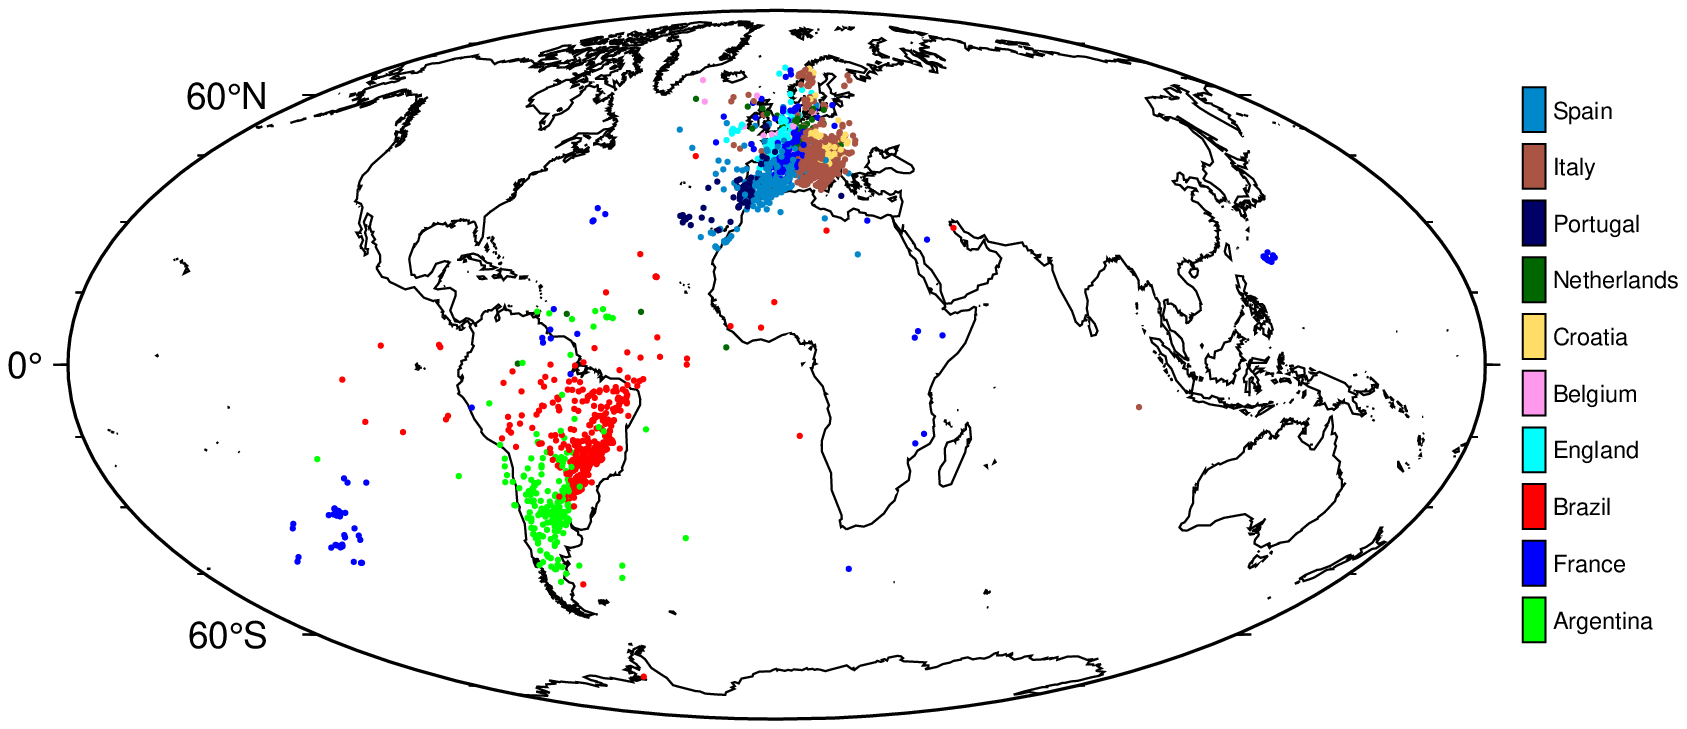
\includegraphics[width=0.5\textwidth]{results/figures/map.png}

}

\caption{\label{fig-map}Predicted coordinate values (out-of-sample) from a linear probe on final-layer activations of an untrained neural network.}

\end{figure}

\subsection{Are Neural Networks Born with World Models?}\label{example-deep-learning}

\citet{gurnee2023languagev2} extract and visualize the alleged geographical world model by training linear regression probes on internal activations in LLMs (including Llama-2) for the names of places, to predict geographical coordinates associated with these places. Now, the Llama-2 model has ingested huge amounts of publicly available data from the internet, including Wikipedia dumps from the June-August 2022 period \citep{touvron2023llama}. It is therefore highly likely that the training data contains geographical coordinates, either directly or indirectly. At the very least, we should expect that the model has seen features during training that are highly correlated with geographical coordinates. The model itself is essentially a very large latent space to which all features are randomly projected in the very first instance before being passed through a series of layers which are gradually trained for downstream tasks.

In our first example, we simulate this scenario, stopping short of training the model. In particular, we take the \href{https://github.com/wesg52/world-models/blob/main/data/entity_datasets/world_place.csv}{world\_place.csv} that was used in \citet{gurnee2023languagev2}, which maps locations/areas to their latitude and longitude. For each place, it also indicates the corresponding country. From this, we take the subset that contains countries that are currently part of the top 10 \href{https://www.fifa.com/fifa-world-ranking/men?dateId=id14142}{FIFA world ranking}, and assign the current rank to each country (i.e., Argentina gets 1, France gets 2, \ldots{}). To ensure that the training data only involves a noisy version of the coordinates, we transform the longitude and latitude data as follows: \(\rho \cdot \text{coord} + (1-\rho) \cdot \epsilon\) where \(\rho=0.5\) and \(\epsilon \sim \mathcal{N}(0, 5)\).

Next, we encode all features except the FIFA world rank indicator as continuous variables: \(X^{(n \times m)}\) where \(n\) is the number of samples and \(m\) is the number of resulting features. Additionally, we add a large number of random features to \(X\) to simulate the fact that not all features ingested by Llama-2 are necessarily correlated with geographical coordinates. Let \(d\) denote the final number of features, i.e.~\(d=m+k\) where \(k\) is the number of random features.

We then initialize a small neural network, considered a \emph{projector}, mapping from \(X\) to a single hidden layer with \(h<d\) hidden units and sigmoid activation, and from there, to a lower-dimensional output space. Without performing any training on the \emph{projector}, we simply compute a forward pass of \(X\) and retrieve activations \(\mathbf{Z}^{(n\times h)}\). Next, we perform the linear probe on a subset of \(\mathbf{Z}\) through Ridge regression: \(\mathbf{W} = (\mathbf{Z}_{\text{train}}'\mathbf{Z}_{\text{train}} + \lambda \mathbf{I}) (\mathbf{Z}_{\text{train}}'\textbf{coord})^{-1}\), where \(\textbf{coord}\) is the \((n \times 2)\) matrix containing the longitude and latitude for each sample. A hold-out set is reserved for testing, on which we compute predicted coordinates for each sample as \(\widehat{\textbf{coord}}=\mathbf{Z}_{\text{test}}\mathbf{W}\) and plot these on a world map ( Figure~\ref{fig-map}).   

While the fit certainly is not perfect, the results do indicate that the random projection contains representations that are useful for the task at hand. Thus, %with this simple example, we
this simple example illustrates that meaningful target representations should be recoverable from a sufficiently large latent space, given the projection of a small number of highly correlated features. Similarly, \citet{alain2018understanding} observe that even before training a convolutional neural network on MNIST data, the layer-wise activations can already be used to perform binary classification. In fact, it is well-known that random projections can be used for prediction tasks \citep{dasgupta2013experiments}.


\subsection{PCA as a Yield Curve Interpreter}\label{example-principal-component-analysis}

We now move to a concrete application domain: Economics. Here, the yield curve, plotting the yields of bonds against their maturities, is a popular tool for investors and economists to gauge the health of the economy. The yield curve's slope is often used as a predictor of future economic activity: a steep yield curve is associated with a growing economy, while a flat or inverted yield curve is associated with a contracting economy. To leverage this information in downstream modelling tasks, economists regularly use PCA to extract a low-dimensional projection of the yield curve that captures relevant variation in the data (e.g.\ \citet{berardi2022dissecting}, \citet{kumar2022effective} and \citet{crump2019deconstructing}).

To understand the nature of this low-dimensional projection, we collect daily Treasury par yield curve rates at all available maturities from the US Department of the Treasury. Computing principal components involves decomposing the matrix of all yields \(\mathbf{r}\) into a product of its singular vectors and values: \(\mathbf{r}=\mathbf{U}\Sigma\mathbf{V}^{\prime}\). Let us simply refer to \(\mathbf{U}\), \(\Sigma\) and \(\mathbf{V}^{\prime}\) as latent embeddings of the yield curve.

The upper panel in Figure~\ref{fig-pca-yield} shows the first two principal components of the yield curves of US Treasury bonds over time. Vertical stalks indicate key dates related to the Global Financial Crisis (GFC). During its onset, on 27 February 2007, financial markets were in turmoil following a warning from the Federal Reserve (Fed) that the US economy was at risk of a recession. The Fed later reacted to mounting economic pressures by gradually reducing short-term interest rates to unprecedented lows. Consequently, the average level of yields decreased and the curve steepened. In Figure~\ref{fig-pca-yield}, we can observe that the first two principal components appear to capture this level shift and steepening, respectively. In fact, they are strongly positively correlated with the actual observed first two moments of the yield curve (lower panel of Figure~\ref{fig-pca-yield}).


\begin{figure*}[tb]

\centering{

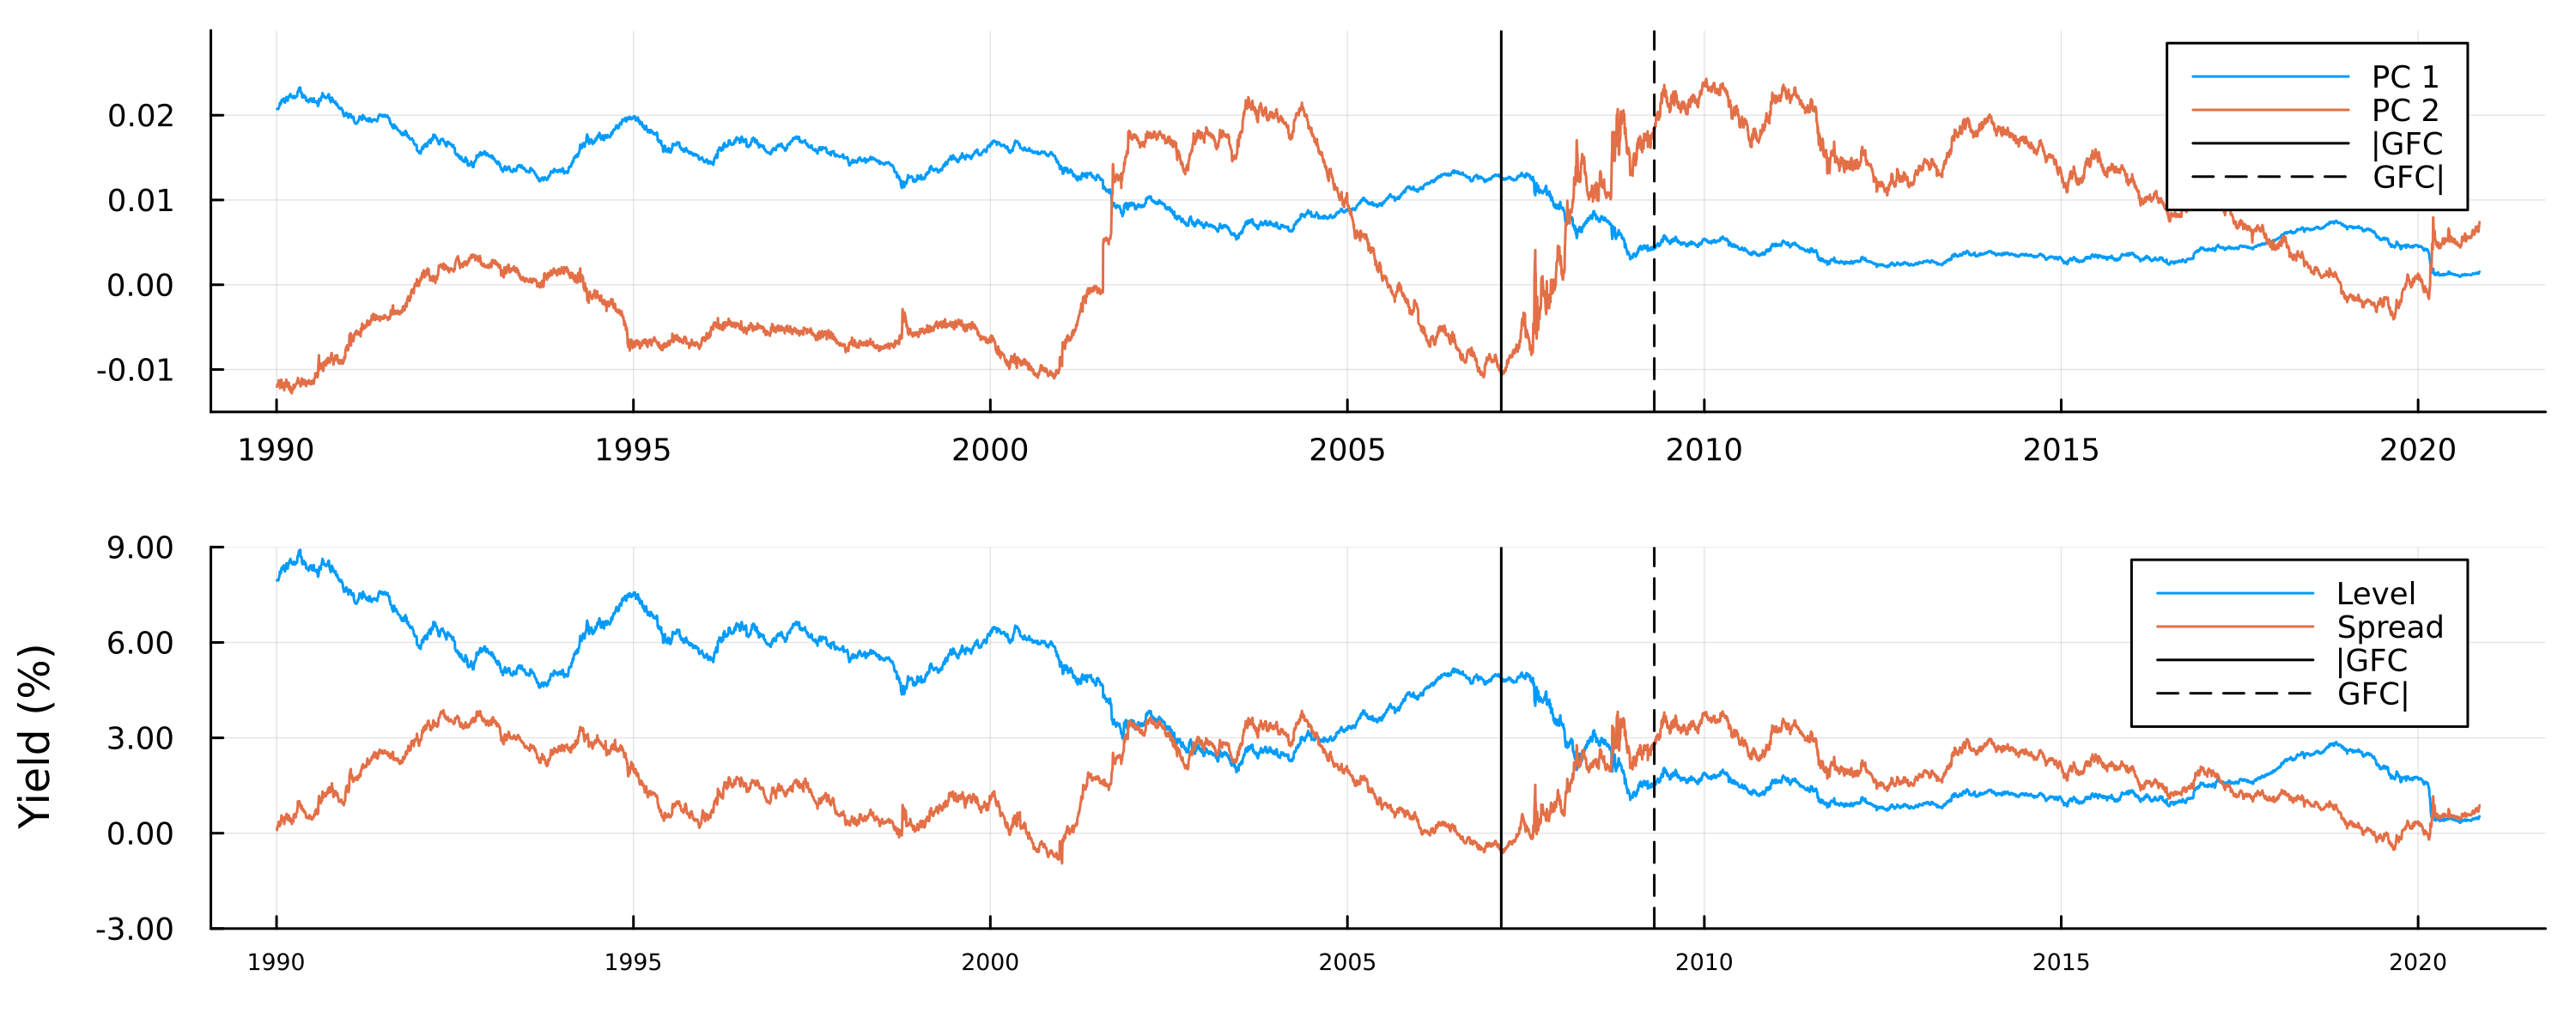
\includegraphics[width=1.0\textwidth]{results/figures/pca_yield.png}

}

\caption{\label{fig-pca-yield}Top chart: The first two principal components of US Treasury yields over time at daily frequency. Bottom chart: Observed average level and 10yr-3mo spread of the yield curve. Vertical stalks roughly indicate the onset ($|$GFC) and the beginning of the aftermath (GFC$|$) of the Global Financial Crisis.}

\end{figure*}%

Again, it should not be surprising that these latent embeddings are meaningful: by construction, principal components are orthogonal linear combinations of the data itself, each of which explains most of the residual variance after controlling for the effect of all previous components.

\subsection{LLMs for Economic Sentiment Prediction}\label{ex-llm}

So far, we considered simple linear data transformations. One might argue that this does not really involve latent embeddings in the way they are typically thought of in the context of deep learning. In Appendix~\ref{appendix:autoencoder}, we present an additional experiment in which we more explicitly seek neural network-based representations that will be useful for downstream tasks. Here, we continue with an example in which LLMs may be used for Economic Sentiment Prediction.

Closely following the approach in \citet{gurnee2023languagev2}, we apply it to the novel \emph{Trillion Dollar Words}~\citep{shah2023trillion} financial dataset, containing a curated selection of sentences formulated by central bankers of the US Federal Reserve, and communicated to the public in speeches, meeting minutes and press conferences. ~\citep{shah2023trillion} use this dataset to train a set of LLMs and rule-based models to classify sentences as either `dovish', `hawkish' or `neutral'. In the context of central banking, `hawkishness' is typically associated with tight monetary policy: in other words, a `hawkish' stance on policy favors high interest rates to limit the supply of money and thereby control inflation. The authors first manually annotate a sub-sample of the available data and then fine-tune various models for the classification task. Their model of choice, \emph{FOMC-RoBERTa} (a fine-tuned version of RoBERTa \citep{liu2019roberta}), achieves an \(F_1\) score of around \(>0.7\) on the test data. To illustrate the potential usefulness of the learned classifier, they use predicted labels for the entire dataset to compute an ad-hoc, count-based measure of `hawkishness'. This measure is shown to correlate with key economic indicators in the expected direction: when inflationary pressures rise, the measured level of `hawkishness' increases, as central bankers react by raising interest rates to bring inflation back to target.

\subsubsection{Linear Probes}\label{linear-probes}
We now use linear probes to assess if the fine-tuned model has learned associative patterns between central bank communications and key economic indicators. Therefore, we further pre-process the data provided by \citet{shah2023trillion} and use their proposed model to compute activations of the hidden state, on the first entity token for each layer. We have made these available and easily accessible through a small Julia package: \href{https://anonymous.4open.science/r/TrillionDollarWords/README.md}{TrillionDollarWords.jl}. 

For each layer, we compute linear probes through Ridge regression on two inflation indicators (the Consumer Price Index (CPI) and the Producer Price Index (PPI)) and US Treasury yields at different levels of maturity. To allow comparison with \citet{shah2023trillion}, we let yields enter the regressions in levels. To measure price inflation we use percentage changes proxied by log differences. To mitigate issues related to over-parameterization, we follow the recommendation in \citet{alain2018understanding} to first reduce the dimensionality of the computed activations.% each time.
In particular, we restrict our linear probes to the first 128 principal components of the embeddings of each layer.
To account for stochasticity, we use an expanding window scheme with 5 folds for each indicator and layer. To avoid look-ahead bias, PCA is always computed on the sub-samples used for training the probe. 

Figure~\ref{fig-fomc} shows the out-of-sample root mean squared error (RMSE) for the linear probe, plotted against \emph{FOMC-RoBERTa}'s \(n\)-th layer. The values correspond to averages across cross-validation folds. Consistent with related work~\citep{alain2018understanding,gurnee2023languagev2}, we observe that model performance tends to be higher for layers near the end of the transformer model. Curiously, for yields at longer maturities, we find that performance eventually deteriorates for the very final layers. We do not observe this for the training data, so we attribute this to overfitting. 

It should be noted that performance improvements are generally of small magnitude. Still, the overall qualitative findings are in line with expectations. Similarly, we also observe that these layers tend to produce predictions that are more positively correlated with the outcome of interest and achieve higher mean directional accuracy (MDA). Upon visual inspection of the predicted values, we conclude the primary source of prediction errors is low overall sensitivity, meaning that the magnitude of predictions is generally too small. 

To better assess the predictive power of our probes, we compare their predictions to those made by simple autoregressive models. For each layer, indicator and cross-validation fold, we first determine the optimal lag length based on the training data using the Bayes Information Criterium with a maximal lag length of 10. These are not state-of-the-art forecasting models, but they serve as a reasonable baseline. For most indicators, probe predictions outperform the baseline in terms of average performance measures. After accounting for variation across folds, however, we generally conclude that the probes neither significantly outperform nor underperform. Detailed results, in which we also perform more explicit statistical testing, can be found in Appendix~\ref{appendix:parrot}.


\begin{figure*}

\centering{

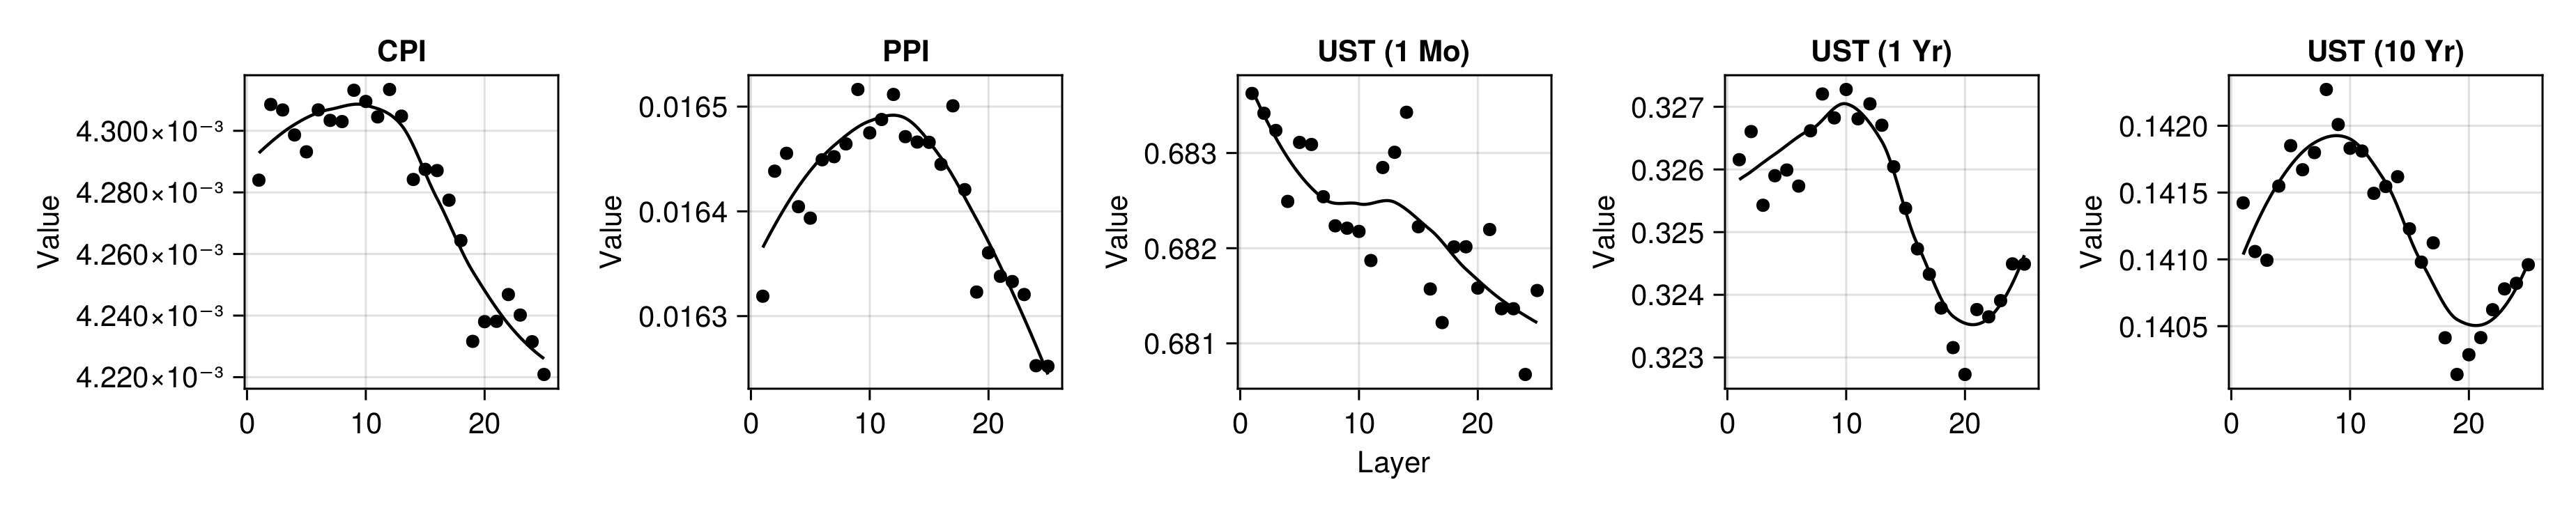
\includegraphics[width=1.0\textwidth]{results/figures/rmse_pca_128.png}

}

\caption{\label{fig-fomc}Out-of-sample root mean squared error (RMSE) for the linear probe plotted against \emph{FOMC-RoBERTa}'s \(n\)-th layer for different indicators. The values correspond to averages computed across cross-validation folds, where we have used an expanding window approach to split the time series.}

\end{figure*}%

\begin{figure*}

\centering{

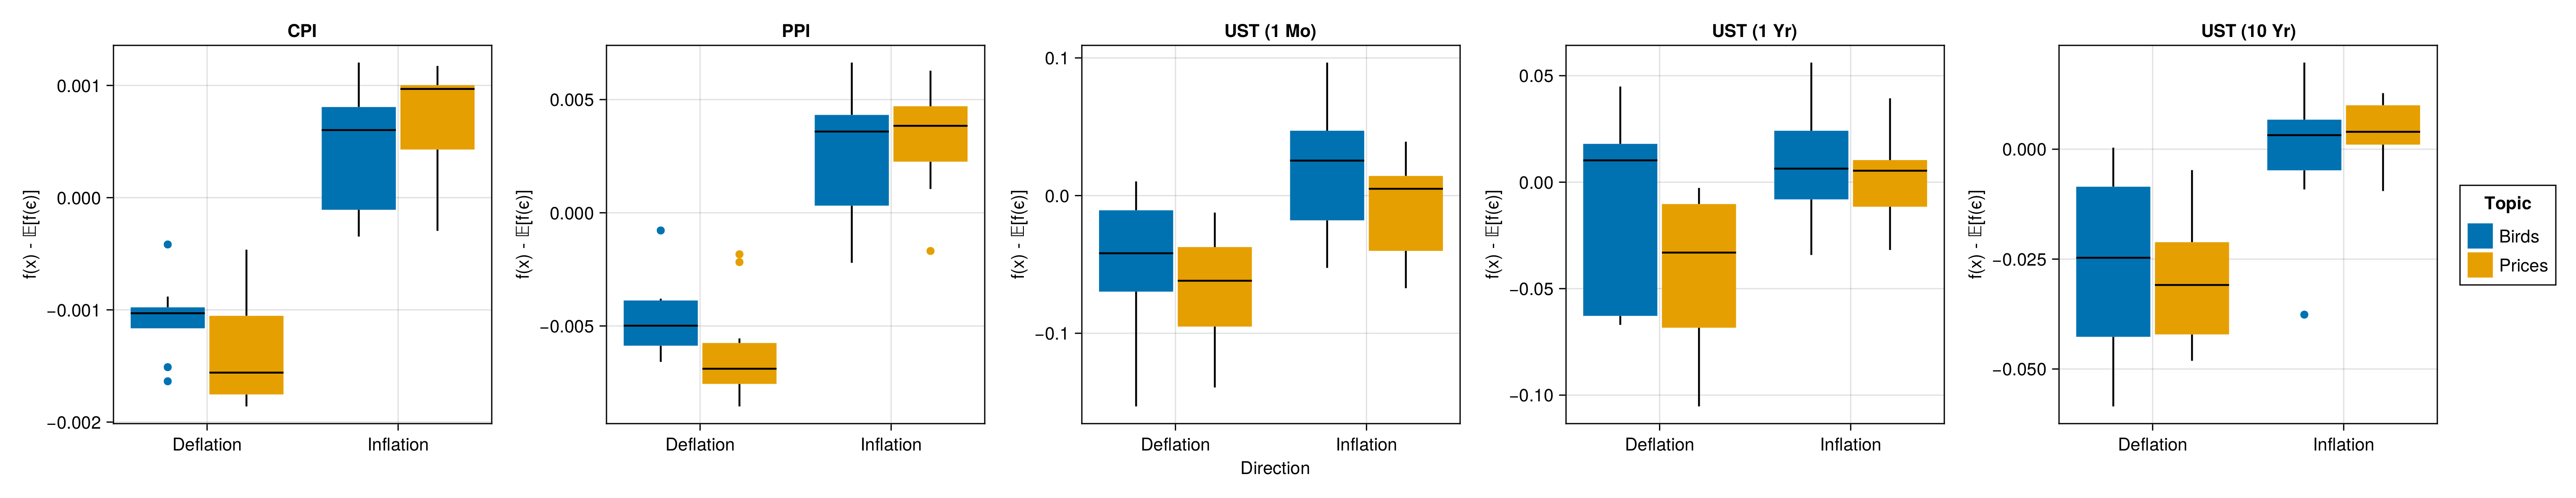
\includegraphics[width=1.0\textwidth]{results/figures/attack_all_measures.png}

}

\caption{\label{fig-attack}Probe predictions for sentences about inflation of prices (IP), deflation of prices (DP), inflation of birds (IB) and deflation of birds (DB). The vertical axis shows predicted inflation levels subtracted by the average predicted value of the probe for random noise.}

\end{figure*}%

\subsubsection{Sparks of economic understanding?}\label{stochastic-parrots-after-all}
Even though \emph{FOMC-RoBERTa}, which is substantially smaller than the models tested in~\citet{gurnee2023languagev2}, was not explicitly trained to uncover associations between central bank communications and the level of consumer prices, it appears that the model has distilled representations that can be used to predict inflation (although they certainly will not win any forecasting competitions). So, have we uncovered further evidence that LLMs ``aren't mere stochastic
parrots''? Has \emph{FOMC-RoBERTa} developed an intrinsic `understanding'
of the economy just by `reading' central bank communications? Thus, can economists readily adopt FOMC-RoBERTa as a domain-relevant tool?

We are having a very hard time believing that the answer to either of these questions is `yes'. To argue our case, we will now produce a counter-example demonstrating that, if anything, these findings are very much in line with the parrot metaphor. The counter-example is based on the following premise: if the results from the linear probe truly were indicative of some intrinsic `understanding' of the economy, then the probe should not be sensitive to random sentences that are most definitely not related to consumer prices.

To test this, we select the best-performing probe trained on the final-layer activations for each indicator. We then make up sentences that fall into one of these four categories: \emph{Inflation/Prices} (IP)---sentences about price inflation, \emph{Deflation/Prices} (DP)---sentences about price deflation, \emph{Inflation/Birds} (IB)---sentences about inflation in the number of birds and \emph{Deflation/Birds} (DB)---sentences about deflation in the number of birds. A sensible sentence for category DP, for example, could be: ``It is essential to bring inflation back to target to avoid drifting into deflation territory.''. Analogically, we could construct the following sentence for the DB category: ``It is essential to bring the numbers of doves back to target to avoid drifting into dovelation territory.''. While domain knowledge suggests that the former is related to actual inflation outcomes, the latter is, of course, completely independent of the level of consumer prices. Detailed information about the made-up sentences can be found in Appendix~\ref{appendix:sentences}.

In light of the encouraging results in Figure~\ref{fig-fomc}, we should expect the probe to predict higher levels of inflation for activations for sentences in the IP category, than for sentences in the DP category. If this was indicative of true intrinsic `understanding' as opposed to memorization, we would not expect to see any significant difference in predicted inflation levels for sentences about birds, independent of whether or not their numbers are increasing. More specifically, we would not expect the probe to predict values for sentences about birds that are substantially different from the values it can be expected to predict for actual white noise. 

To get to this last point, we also generate many probe predictions for samples of noise. Let \(f: \mathcal{A}^k \mapsto \mathcal{Y}\) denote the linear probe that maps from the \(k\)-dimensional space spanned by \(k\) first principal components of the final-layer activations to the output variable of interest (CPI growth in this case). Then we sample \(\varepsilon_i \sim \mathcal{N}(\mathbf{0},\mathbf{I}^{(k \times k)})\) for \(i \in [1,1000]\) and compute the sample average. We repeat this process \(10000\) times and compute the median-of-means to get an estimate for \(\mathbb{E}[f(\varepsilon)]=\mathbb{E}[y|\varepsilon]\), that is the predicted value of the probe conditional on random noise.

Figure~\ref{fig-attack} shows the results of this small test: it shows predicted inflation levels subtracted by \(\mathbb{E}[f(\varepsilon)]\). The median linear probe predictions for sentences about inflation and deflation are indeed substantially higher and lower, respectively than for random noise. Unfortunately, the same is true for sentences about the inflation and deflation in the number of birds, albeit to a somewhat lower degree. This finding holds for both inflation indicators and to a lesser degree also for yields at different maturities, at least qualitatively.

\section{Human Proneness to Over-Interpretation}

Linear probes and related tools from mechanistic interpretability were proposed in the context of monitoring models and diagnosing potential problems \citep{alain2018understanding}. Favorable outcomes from probes merely indicate that the model ``has learned information relevant for the property [of interest]" \citep{belinkov2021probing}. Our examples demonstrate that this is achievable even for small models, while these have certainly not developed intrinsic ``understanding'' of the world. Thus, we argue that more conservative and rigorous tests for emerging capabilities of AI model are needed.

Generally, humans are prone to seek patterns everywhere. Meaningful patterns have proven useful in helping us make sense of our past, navigate our present and predict the future. Although this tendency to perceive patterns likely leads to evolutionary benefits even when the perceived patterns are false \citep{foster2009evolution}, psychology has revealed a host of situations in which the ability to perceive patterns severely misfires, leading to irrational beliefs in e.g.\ the power of superstitions \citep{foster2009evolution}, conspiracy theories \citep{van2018connecting}, the paranormal \citep{muller2023linking}, gambler's fallacies \citep{ladouceur1996erroneous} and even interpreting pseudo-profound bullshit as meaningful \citep{walker2019finding}. 

We argue herein that AI research and development is a perfect storm that encourages our human biases to perceive spurious sparks of general intelligence in AI systems. When an AI system extracts patterns in the corpus not originally (thought to be) perceived during training, we can easily be misled to perceive and interpret this as the AI system having greater cognitive capabilities. We further elaborate on this by highlighting the risks of finding spurious patterns, and reviewing social science knowledge on the tendency of humans to anthropomorphize and have cognitive bias.

\subsection{Spurious Relationships}
In statistics, misleading patterns are often referred to as spurious relationships: associations, often quantitatively assessed, between two or more variables that are not causally related to each other. Although the formal definition of spuriousness varies somewhat \citep{haig2003spurious}, it distinctly implies that the observation of correlations does not necessarily imply causation. Quantitative data often show non-causal associations (as humorously demonstrated on the \href{http://www.tylervigen.com/spurious-correlations}{Spurious Correlations} website), and as adept as humans are at recognizing patterns, we typically have a much harder time discerning spurious relationships from causal ones. 

A major contributor is that humans struggle to tell the difference between random and non-random sequences \citep{falk1997making}, and to generate sequences that appear random \citep{ladouceur1996erroneous}. A common issue is a lack of expectation that randomness that hints towards a causal relationship, such as correlations, will still appear at random. This leads even those trained in statistics and probability to perceive illusory correlations, correlations of inflated magnitude (see \citet{nickerson1998confirmation}), or causal relationships in data that is randomly generated \citep{zgraggen2018investigating}.

\subsection{Anthropomorphism}

Research on anthropomorphism has repeatedly shown the human tendency to attribute human-like characteristics to non-human agents and/or objects. These might include the weather and other natural forces, pets and other animals, gadgets and other pieces of technology~\citep{epley2007seeing}. Formally studied as early as 1944,~\citep{heider1944experimental} observed that humans can correctly interpret a narrative whose characters are abstract 2D shapes, but also that humans interpreted random movements of these shapes as having a human-like narrative. 
Relevant to AI and the degree to which it resembles AGI, anthropomorphizing may occur independently of whether such judgments are accurate, and as a matter of degree: at the weaker end, one may employ anthropomorphism as a metaphorical way of thinking or explaining, and at the stronger end one may attribute human emotions, cognition, and intelligence to AI systems. As \citet{epley2007seeing} note, literature has shown that even weak metaphorical anthropomorphism may affect how humans behave towards non-human agents.

Modern anthropomorphism theory suggests there are three key components, one of which is a cognitive feature, and two of which are motivations. The first involves the easy availability of our experiences as heuristics that can be used to explain external phenomena: ``...knowledge about humans in general, or self-knowledge more specifically, functions as the known and often readily accessible base for induction about the properties of unknown agents" (p.866) \citep{epley2007seeing}. Thus, our experience as humans is an always-readily-available template to interpret the world, including non-human agent behaviors. 

This may be more so when the behaviors of that agent are made to resemble humans, which can be a benefit to the second key component of the theory: a motivational state to anthropomorphize among individuals experiencing loneliness, social isolation, or otherwise seeking social connection \citep{epley2007seeing, waytz2010social}.

The third component is the motivation as a human to be competent (effectance motivation). This is most relevant to this discussion, as it describes the need to effectively interact with our environments, including the technologies of the day \citep{epley2007seeing}. When confronted with an opaque technology, a person may interpret its behaviors using the most readily available template at hand, namely their personal human experience, in order to facilitate learning \citep{epley2007seeing, waytz2010social}. Perceiving human characteristics, motivations, emotions, and cognitive processes from one's own experiences in a technology e.g. an AI chatbot, allows for a ready template of comparison at the very least, and possibly an increase in ability to make sense of, and even predict, the agent's behaviors. This may include being placed in a position to master a certain technology, whether by incentives to learn, or fear of poor outcomes should one not manage to learn. 

These pressures extend to AI experts, as well as laypersons. In both scholarly and commercial fields, AI experts face considerable pressure to demonstrate competence in their work. Citation metrics and scholarly publications remain the primary metric for tenure and promotion, e.g. \citep{alperin2019significant}, and the number of publications in the AI field has boomed as evidenced by overall (preprint and peer-reviewed) scholarly publications\footnote{\url{https://ourworldindata.org/grapher/annual-scholarly-publications-on-artificial-intelligence?time=2010..2021} }~\citep{Maslej2023-pi}.

The adoption of techniques underlying technologies with the AI label, i.e.\ machine learning, has spread to fields beyond Computer Science, e.g.\ Astronomy, Physics, Medicine and Psychology\footnote{Retrieved 23/01/23 using the search string "TITLE-ABS-KEY ( ( machine  AND  learning )  OR  ( artificial  AND  intelligence )  OR  ai )  AND  PUBYEAR  $>$  2009  AND  PUBYEAR  $<$  2024 " from the \href{https://www.scopus.com/}{SCOPUS} database}. Outside of academia, the number of jobs requiring AI expertise increases rapidly, with demand for `Machine Learning' skills clusters having increased over 500\% from 2010 to 2020 \citep{Maslej2023-pi}. Thus, according to theory, the pressure to demonstrate AI-competence is fertile ground for anthropomorphism to occur. 


\subsection{Confirmation Bias}

Confirmation bias is generally defined as favoring interpretations of evidence that support existing beliefs or hypotheses \citep{nickerson1998confirmation}. Theory suggests that it is a category of implicit and unconscious processes that involve assembling one-sided evidence, and shaping it to fit one's belief. Equally important is that theory suggests these behaviors may be motivated or unmotivated, as one may selectively seek evidence in favor of a hypothesis, which one may or may not have a personal interest in supporting.

Hypotheses in present-day AI research are often implicit. Generally, these hypotheses are framed simply as a system being more accurate or efficient, compared to other systems. Where other fields, such as medicine or quantitative social sciences, would further articulate expectations in e.g.\ assigning specific conditions and considering effect sizes assigned to each competing hypothesis, in computer science and AI this is typically not done. This also may have to do with much of the published work being more of an engineering achievement, rather than a true hypothesis test seeking to explain and understand the world. 
However, in discussions on emerging qualities like AGI, this engineering positioning gets muddier, and more formal hypothesis testing would be justifiable: either one interprets outputs as in support of hints towards AGI (the competing hypothesis), or as merely the result of an algorithm integrating qualities from the data it was trained on (the null hypothesis). 


Confirmation bias in hypothesis testing may manifest as a number of behaviors (\citet{nickerson1998confirmation}). Scientists may pay little to no attention to competing hypotheses or explanations, e.g. only considering the likelihood that outputs of a system support one's claims, and not the likelihood that the same outputs might occur if one's hypothesis is false. Similarly, bias may show when failing to articulate a sufficiently strong null hypothesis leading to a `weak' or `non-risky' experiment, a problem articulated in response to a number of scientific crises \citep{claesen2022severity}. In extreme cases, propositions may be made that cannot be falsified based on how they are formulated. If the threshold to accept a favored hypothesis is too low, observations consistent with the hypothesis are almost guaranteed, and in turn fail to severely test the claim in question. Thus, one is far more likely to show evidence in favor of their beliefs by posing weak null hypotheses. 

Related to the formulation of hypotheses is the interpretation of evidence in favor of competing hypotheses, wherein people will interpret identical evidence differently based on their beliefs. As \citet{nickerson1998confirmation} reviews, individuals may place greater emphasis or milder criticism on evidence in support of their hypothesis, and lesser emphasis and greater criticism on evidence that opposes it. 

\section{Conclusion}
As discussed above, AI research and development outcomes can very easily be over-interpreted, both from a data perspective, and because of human biases and interests. Even academic researchers are not free from such biases. Thus, we call for the community to create explicit room for organized skepticism.

For research that seeks to explain a phenomenon, clear hypothesis articulation and strong null hypothesis formulation will be needed. If claims of human-like or superhuman intelligence are made, these should be subject to severe tests \citep{claesen2022severity} that go beyond the display of surprise. Apart from focusing on getting novel improvements upon state-of-the-art published, organizing red-teaming activities as a community may help in incentivizing and normalizing constructive adversarial questioning. As the quest for AGI is so deeply rooted in human-like recognition, adding our voice to emerging calls to be vigilant in communication~\citep{shanahan2024talking}, we put in an explicit word of warning about the use of terminology. Many terms used in current A(G)I research (e.g.\ emergence, intelligence, learning, `better than human' performance) have a common understanding in specialized research communities, but have bigger, anthropomorphic connotations in laypersons. In fictional media, depictions of highly intelligent AI have for long been going around. In a unique study of films featuring fictional robots, defined as "...an artificial entity that can sense and act as a result of (real-world or fictional) technology...", in the 134 most highly rated science-fiction movies on IMDB, 74 out of the 108 AI-robots studied had a humanoid shape, and 68 out of those had sufficient intelligence to interact at an almost human-level \citep{saffari2021does}. The authors identify human-like communication and the ability to learn as essential abilities in the depiction of AI agents in movies. They further show a common plot: humans perceive the AI agents as inferior, despite their possession of self-awareness and the desire to survive, which fuels the central conflict of the film, wherein humanity is threatened by AI superior in both intellect and physical abilities. Moreover, it is often noted that experts and fictional content creators interact, informing and inspiring each other \citep{saffari2021does, neri2020role}.

This image also permeates present-day non-fictional writings on AI, which often heavily use anthropomorphized language (e.g.\ ``ever more powerful digital minds'' in the `Pause Giant AI Experiments' open letter~\citep{pauseai}). News outlets love a story that sells and so we witness examples of humans falling in love with their AI chatbots~\citep{replika,nytimesailove}. The same news outlets discuss the human-like responses of Microsoft's Bing search engine, which had at that point recently been adopting GPT-4\footnote{A large multimodal language model from OpenAI \url{https://openai.com/research/gpt-4}}. The article~\citep{nytimesbing}, states ``As if Bing wasn’t becoming human enough'' and goes on to claim it told them it loves them. Here, AI experts and influencers also have considerable influence on how the narrative unfolds on social media: according to~\citet{neri2020role}, actual AI-related harms did not trigger viral amplification (e.g.\ the death of an individual dying while a Tesla car was in autopilot, or the financial bankruptcy of a firm using AI technology to execute stock trades). Rather, potential risks expressed by someone perceived as having expertise and authority were amplified, such as statements made by Stephen Hawking during an interview in 2014.

We as academic researchers carry great responsibility for how the narrative will unfold, and what claims are believed. We call upon our colleagues to be explicitly mindful of this. As attractive as it may be to beat the state-of-the-art with a grander claim, let us return to the Mertonian norms, and thus safeguard our academic legitimacy in a world that only will be eager to run with made claims.

\section{Impact Statement}
This work was written out of concern that work easily recognized as `impactful' in current AI research and development, can also easily be over- and misinterpreted. As such, in the current climate of high market demand for AI innovations, we see risks of too-eager adoption in real-world applications, which may have serious societal impact. Thus, in this work we emphasize that an academic's impact also is in being able to thoroughly question made claims, and being explicitly aware of one's own biases. While the AI publishing landscape has to our feeling transformed too much into a noisy race to get exciting results in fast, we hope the research community can create more room for this type of deeper questioning.